\documentclass[8pt]{beamer}
\usepackage{gillsans}
\usepackage{hoefler}
\renewcommand{\rmdefault}{HoeflerText}
\usepackage{textpos}

\setbeamertemplate{navigation symbols}{}
\setbeamertemplate{itemize item}{$\bullet$}
\setbeamercolor{item}{fg=black}

\usepackage{soul}
\sodef\expand{}{.08em}{.5em}{.37em plus.1em minus.14em}
\newcommand{\expandUP}[1]{\MakeUppercase{\expand{#1}}}

\begin{document}
\nonfrenchspacing
\begin{frame}[plain]
  \begin{textblock*}{20mm}[1,1](114mm,91mm)
    
\includegraphics[width=\textwidth]{bdcco}
  \end{textblock*}

\vspace{15pt}
\vspace{5pt}
  \begin{center}
    {\Large\bf \expandUP{Biodiversity Coffee Co-op}}
    \rule{.9\textwidth}{1px}
  \end{center}

\rm

Each shot is \$0.35.  Mark down one tick for each shot of espresso you
consume, regardless of the size (each one has the same amount of
espresso, just more or less water).  5c from each cup is donated to
the Nature Trust of BC.

\vspace{6pt}

Milk is an extra \$0.15 extra per shot (total \$0.50 per shot).
\\Tick the ``no milk'' column if you \textit{do not} want to use the
co-op provided milk.

\vspace{10pt}

\small

Your account balance is shown, if the number is \textbf{bolded}, you
owe money!\\
Bring cash contributions to Rich in room 312.

\vspace{10pt}
If your name is not yet on the list, please add it to the bottom. 

\vspace{6pt}
Email Rich (\texttt{fitzjohn@zoology.ubc.ca}) if there is a problem or
we are out of coffee.

%\vspace{10pt}
{\footnotesize
  \begin{itemize}
  \item In the last three ``months'' (30 January to 13 April to 12
    June) we consumed 3,302 and 2,188 coffees, 2,941 and 2,078 of
    which were paid for (89\% and 95\%).
    % \item Track your consumption and balance online:\\
    %   \url{http://www.zoology.ubc.ca/~fitzjohn/coffee}\\
  \item Per-person coffee consumption per career stage:
  \end{itemize}
}

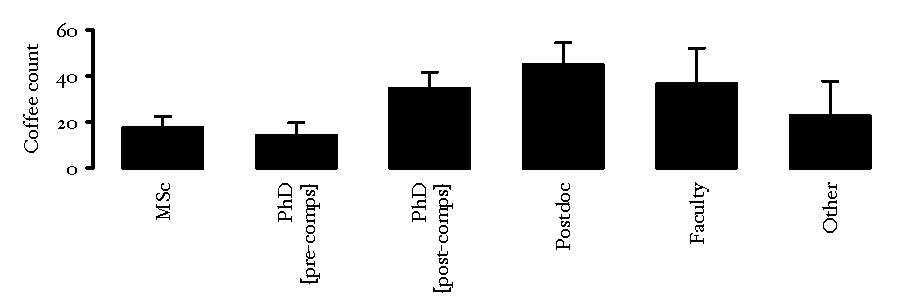
\includegraphics[width=.7\textwidth]{201206-coffee-by-stage}
\vspace{45pt}

\end{frame}

\end{document}

%%% Local Variables: 
%%% mode: latex
%%% TeX-PDF-mode: t
%%% End: 
